All mutators produce mutations with type-level mistakes, but not all such
mutations necessarily represent interesting debugging scenarios. Running a
mutation may not raise a run-time error, though produce the wrong
outputs---something the rational programmer may not recognize and certainly
cannot use for a debugging session. Even if the program execution ends in an
exceptional state, it may do so too quickly; for example, the first-order export
checks of Natural may catch the error and point directly to the faulty module.

To avoid these pitfalls, an \emph{interesting debugging scenario} is
defined as a mutation that satisfies three conditions.  First, {\em
the mutation is rejected by the type checker when all missing type
annotations are restored\/}. This first criterion validates that the
debugging scenario concerns an impedance mismatch.

Second, {\em it produces a run-time exception under Erasure as-is\/}, which
ensures that it is detectable under all three semantics.  Whether a scenario
produces a run time error largely depends on the underlying semantics but
\citet{gfd-oopsla-2019} show that a run-time error under Erasure implies a run
time error under both Transient and Natural. Thus the criterion aligns
interesting debugging scenarios with the lowest denominator, Erasure. It
excludes from consideration the most complex scenarios where only Natural or
Transient can detect a mistake and Erasure is powerless.

{\bf Note} While this choice favors Erasure over Transient and Natural and, for
the same reason, Transient over Natural, some form of bias towards one or the
other semantics is unavoidable. Tipping the scales in favor of the theoretically
weakest semantics yields the most stable results. See
section~\ref{sec:discussion} for some further discussion of this choice.

Third, {\em the exception's stack trace mentions at least three
distinct components\/}, meaning the scenario demands a sufficiently
sophisticated debugging effort: one due to the interaction between the
buggy portion of the program with the rest of the program.  In these
cases, the rational programmer must examine at least modules to locate
the source of the faulty interaction.  In technical terms, if the
stack trace mentions at least two distinct components, the bug should
be revealed by the run-time checks governing an interaction. A third
component is required because all benchmark programs include a driver
component, which is guaranteed to be in the stack trace. In essence,
this last criterion excludes a large number of trivial-to-debug
scenarios that error immediately when their mutated component is
evaluated.

%\begin{figure*}
%  \centering
%  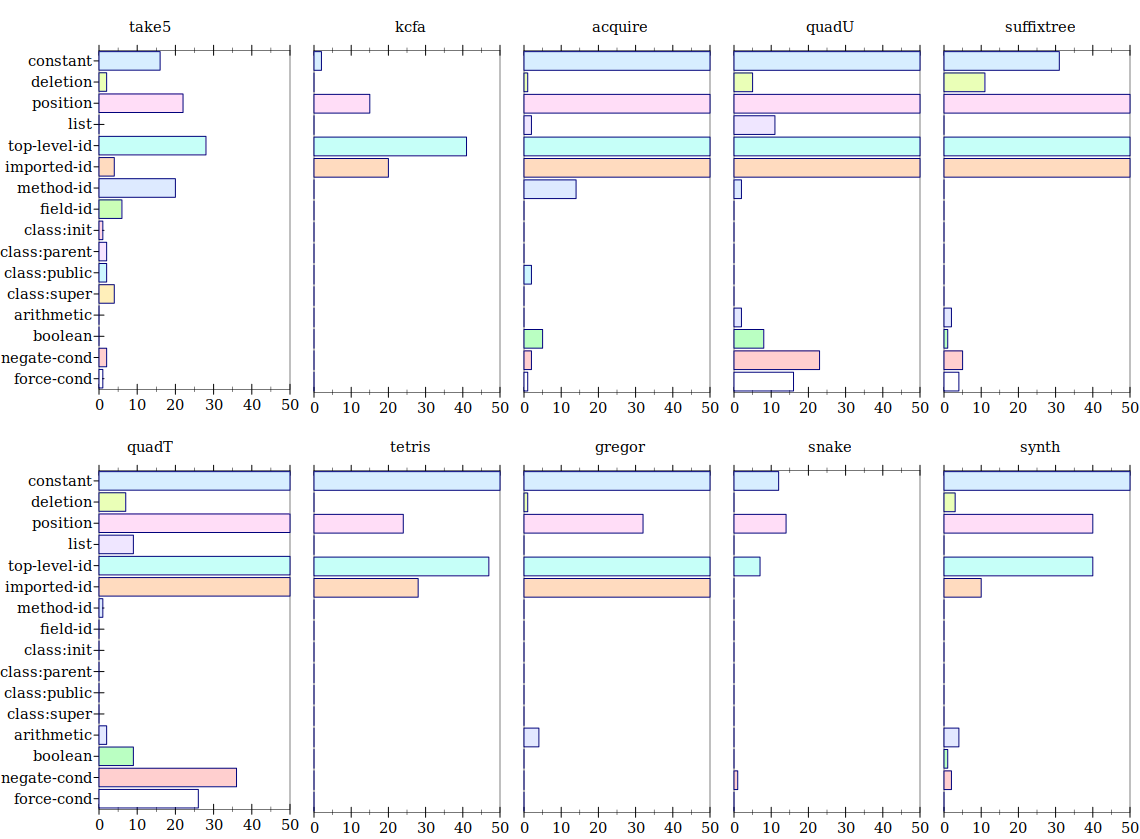
\includegraphics[scale=0.35]{./plots/mutant-breakdown}
%  \caption{Interesting debugging scenarios produced by our mutators. Counts are cut off at 50.}
%  \label{fig:mutant-breakdown}
%\end{figure*}

The definition of interesting debugging scenarios creates a powerful filter. At
a high level, the mutators produce 16,800 mutants with at least one interesting
debugging scenario each across all of benchmarks.  Broken down by benchmark, the
mutators produce at least 40 interesting scenarios for every benchmark, and
these scenarios originate from at least four different mutators per benchmark.
Thus, the mutators result in a sizable and diverse population of scenarios for
every benchmark.  Furthermore, every mutator contributes scenarios to at least
one benchmark.  Note, though, that some mutators apply only to a few benchmarks,
because they target rather specific features.  For instance, the class-focused
mutators are mainly effective in \texttt{take5}, because it makes the most
extensive use of object-oriented Racket features.
